\documentclass[border=3pt,tikz]{standalone}
\usepackage{amsmath,amssymb}
\usepackage{newtxtext,newtxmath}
\usetikzlibrary{arrows.meta,positioning,fit,backgrounds,calc,shapes.geometric}

\begin{document}
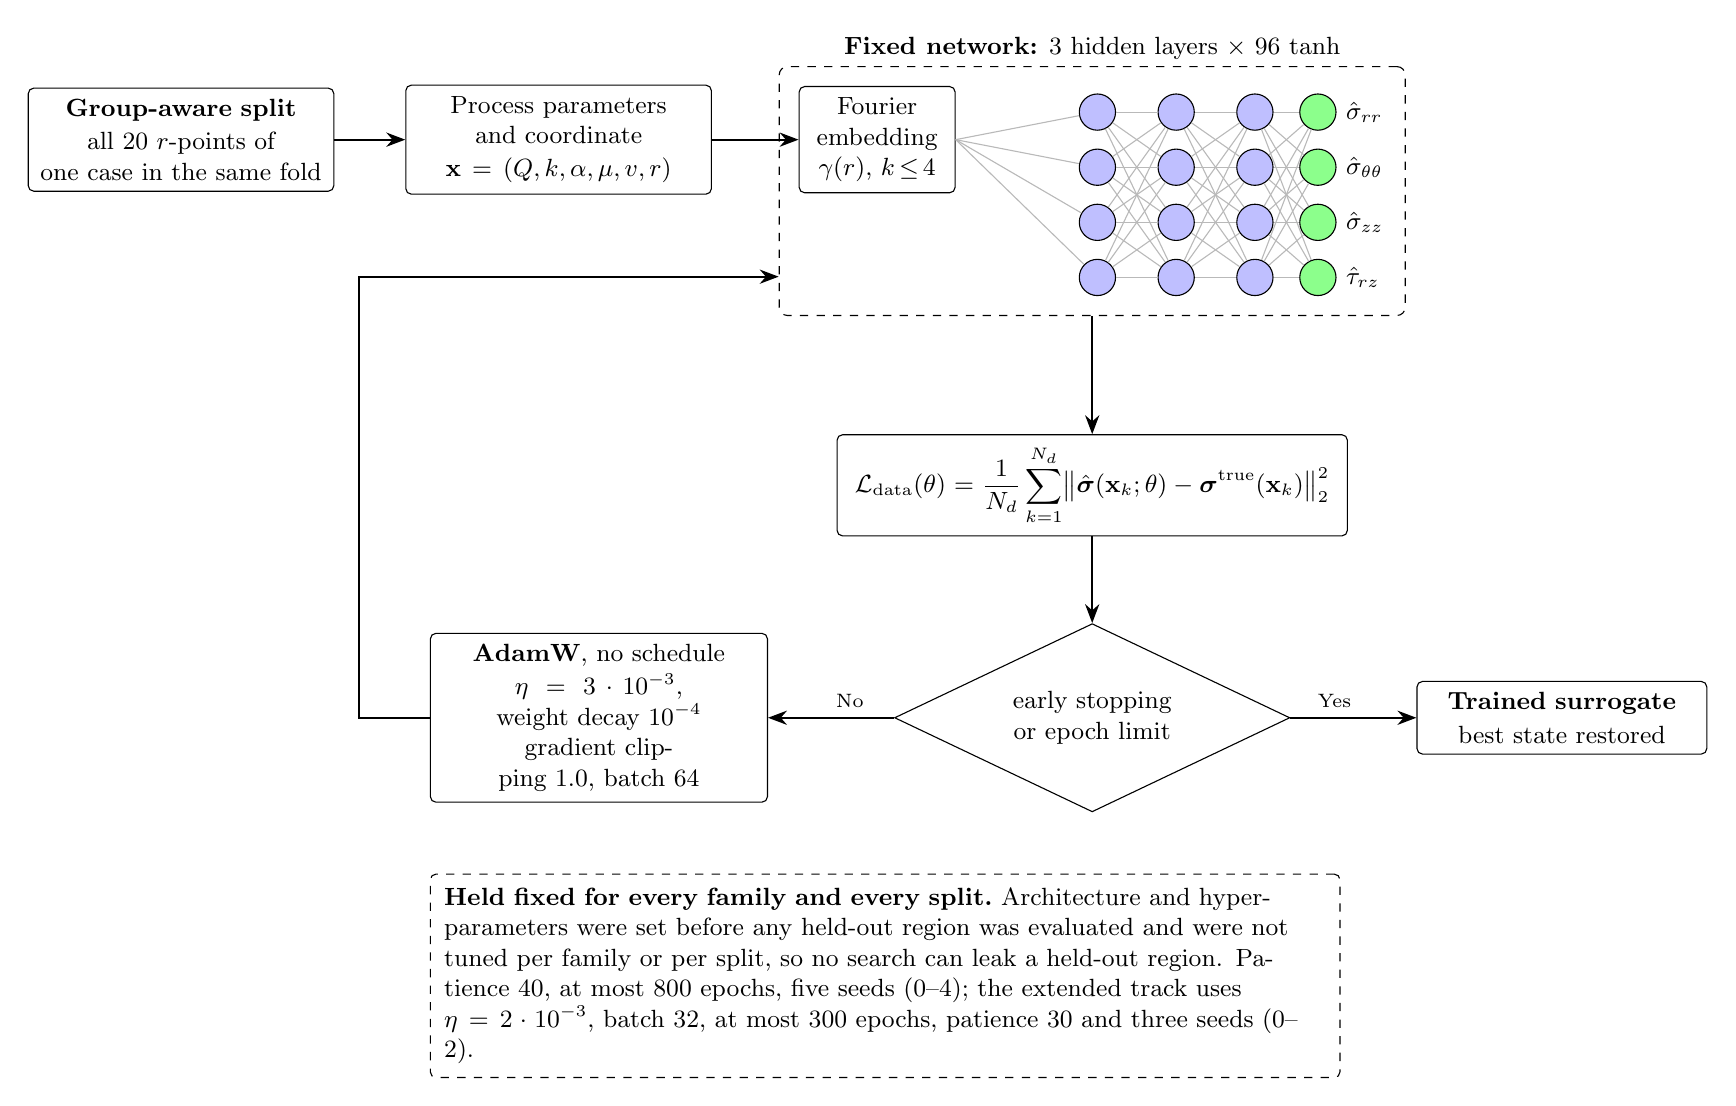
\begin{tikzpicture}[
  font=\small,
  >={Stealth[length=2.4mm]},
  box/.style   ={draw, rounded corners=2pt, align=center, inner sep=4pt, minimum height=9mm},
  wide/.style  ={box, text width=36mm},
  dec/.style   ={draw, diamond, aspect=2.1, align=center, inner sep=1pt},
  note/.style  ={draw, dashed, rounded corners=2pt, align=left, inner sep=5pt},
  lnk/.style   ={->, thick},
  group/.style ={draw, dashed, rounded corners=3pt, inner sep=7pt},
  neuron/.style={circle, draw, minimum size=4.6mm, inner sep=0pt},
]

%% ---------------- input chain ----------------
\node[wide] (split) {\textbf{Group-aware split}\\[1pt]
  all 20 $r$-points of\\ one case in the same fold};

\node[wide, right=9mm of split] (inp) {Process parameters\\ and coordinate\\[1pt]
  $\mathbf{x}=(Q,k,\alpha,\mu,v,r)$};

%% ---------------- network ----------------
\node[box, right=11mm of inp, text width=17mm] (fe)
  {Fourier\\ embedding\\ $\gamma(r)$, $k\!\le\!4$};

\foreach \l in {1,2,3}{
  \foreach \i in {1,2,3,4}{
    \node[neuron, fill=blue!25] (h\l\i) at ($(fe.east)+(8mm+\l*10mm, 10.5mm-\i*7mm)$) {};
  }
}
\foreach \i in {1,2,3,4}{
  \node[neuron, fill=green!45] (o\i) at ($(fe.east)+(46mm, 10.5mm-\i*7mm)$) {};
}
\node[right=0.8mm of o1, inner sep=1pt] (l1) {$\hat\sigma_{rr}$};
\node[right=0.8mm of o2, inner sep=1pt] (l2) {$\hat\sigma_{\theta\theta}$};
\node[right=0.8mm of o3, inner sep=1pt] (l3) {$\hat\sigma_{zz}$};
\node[right=0.8mm of o4, inner sep=1pt] (l4) {$\hat\tau_{rz}$};

\foreach \i in {1,2,3,4}{\draw[gray!55, thin] (fe.east) -- (h1\i);}
\foreach \l [evaluate=\l as \n using int(\l+1)] in {1,2}{
  \foreach \i in {1,2,3,4}{\foreach \j in {1,2,3,4}{\draw[gray!55, thin] (h\l\i) -- (h\n\j);}}}
\foreach \i in {1,2,3,4}{\foreach \j in {1,2,3,4}{\draw[gray!55, thin] (h3\i) -- (o\j);}}

\begin{scope}[on background layer]
  \node[group, fit=(fe)(h11)(h34)(l1)(l4), label={[yshift=-1pt]above:\textbf{Fixed network:} 3 hidden layers $\times$ 96 $\tanh$}] (net) {};
\end{scope}

\draw[lnk] (split) -- (inp);
\draw[lnk] (inp) -- (fe);

%% ---------------- loss ----------------
\node[box, below=15mm of net.south, text width=62mm] (loss)
  {$\displaystyle \mathcal{L}_{\mathrm{data}}(\theta)=\frac{1}{N_d}\sum_{k=1}^{N_d}
    \bigl\|\hat{\boldsymbol\sigma}(\mathbf{x}_k;\theta)-\boldsymbol\sigma^{\mathrm{true}}(\mathbf{x}_k)\bigr\|_2^2$};

\draw[lnk] (net.south) -- (loss.north);

%% ---------------- stopping rule ----------------
\node[dec, below=11mm of loss, text width=34mm] (stop)
  {early stopping\\ or epoch limit};
\draw[lnk] (loss) -- (stop);

\node[wide, left=16mm of stop, text width=40mm] (opt)
  {\textbf{AdamW}, no schedule\\[1pt]
   $\eta=3\cdot10^{-3}$, weight decay $10^{-4}$\\
   gradient clipping 1.0, batch 64};
\draw[lnk] (stop) -- node[above, pos=0.35, font=\scriptsize] {No} (opt);
\coordinate (back) at ($(net.south west)+(0,5mm)$);
\draw[lnk] (opt.west) -- ++(-9mm,0) |- (back);

\node[wide, right=16mm of stop, text width=34mm] (done)
  {\textbf{Trained surrogate}\\[1pt] best state restored};
\draw[lnk] (stop) -- node[above, pos=0.35, font=\scriptsize] {Yes} (done);

%% ---------------- fixed-configuration note ----------------
\node[note, below=9mm of opt.south west, anchor=north west, text width=112mm] (fix)
  {\textbf{Held fixed for every family and every split.}\ Architecture and
   hyperparameters were set before any held-out region was evaluated and were not
   tuned per family or per split, so no search can leak a held-out region. Patience 40,
   at most 800 epochs, five seeds (0--4); the extended track uses
   $\eta=2\cdot10^{-3}$, batch 32, at most 300 epochs, patience 30 and three seeds (0--2).};

\end{tikzpicture}
\end{document}
